\documentclass[tikz,border=8pt]{standalone}
% Shared look for every TikZ diagram. Load with \input{../../tools/tikz-style.tex}
\usepackage[T1]{fontenc}
\usepackage{lmodern}
\renewcommand{\sfdefault}{lmr}  % diagrams use the same serif as the text
\usetikzlibrary{arrows.meta, positioning, shapes.geometric, calc, fit, backgrounds}
\definecolor{cblue}{HTML}{4C78A8}
\definecolor{corange}{HTML}{F58518}
\definecolor{cgreen}{HTML}{54A24B}
\definecolor{cred}{HTML}{E45756}
\definecolor{cpurple}{HTML}{B279A2}
\definecolor{cgrey}{HTML}{6B6B6B}
\tikzset{
  every picture/.style={font=\sffamily, line width=1.2pt},
  box/.style={draw=#1, fill=#1!12, rounded corners=4pt, align=center, inner sep=7pt, minimum height=1.1cm},
  box/.default=cgrey,
  arrow/.style={-{Stealth[length=3mm]}, draw=cgrey, line width=1.4pt},
  title/.style={font=\sffamily\bfseries\Large},
  note/.style={font=\sffamily\small, text=cgrey, align=center},
}
\AtBeginDocument{\hyphenpenalty=10000 \exhyphenpenalty=10000}

\begin{document}
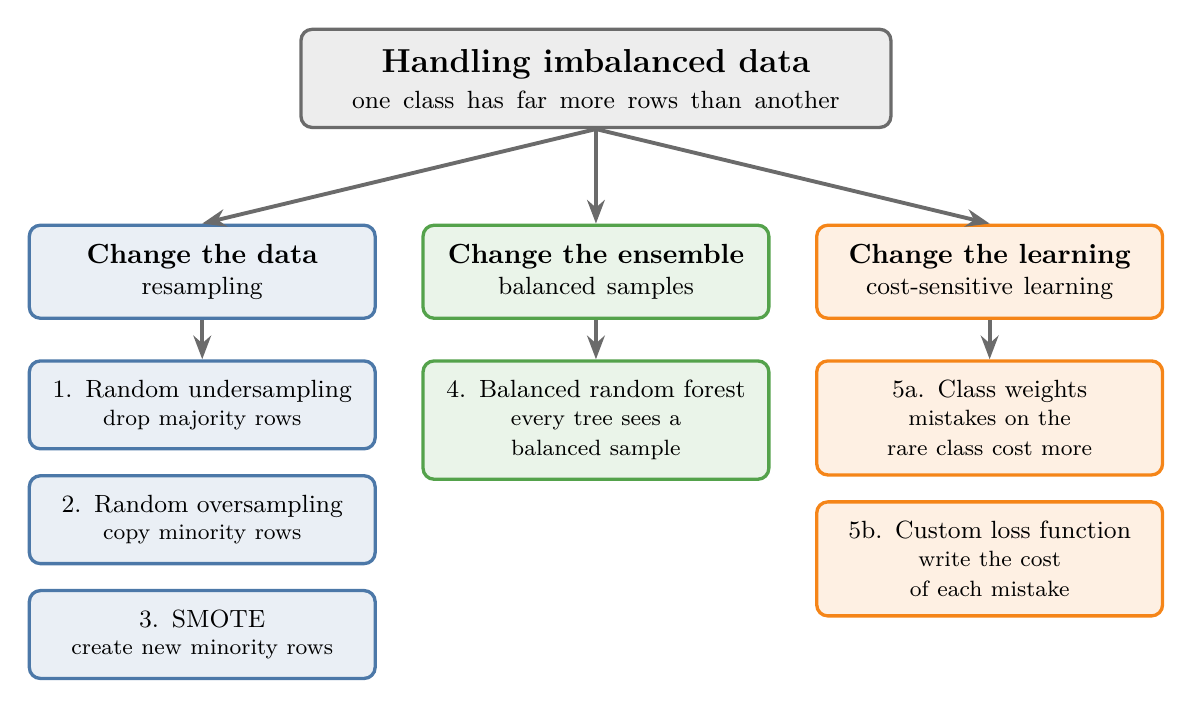
\begin{tikzpicture}[node distance=0.6cm,
  leaf/.style={box=#1, text width=3.9cm, font=\sffamily\small},
  head/.style={box=#1, text width=3.9cm, font=\sffamily\bfseries}]
  \node[box=cgrey, font=\sffamily\bfseries\large, text width=7cm] (top) {Handling imbalanced data\\[-1pt]\normalfont\small one class has far more rows than another};
  \node[head=cblue, anchor=north] (rs) at ($(top.south)+(-5,-1.2)$) {Change the data\\[-1pt]\normalfont\small resampling};
  \node[head=cgreen, anchor=north] (en) at ($(top.south)+(0,-1.2)$) {Change the ensemble\\[-1pt]\normalfont\small balanced samples};
  \node[head=corange, anchor=north] (cs) at ($(top.south)+(5,-1.2)$) {Change the learning\\[-1pt]\normalfont\small cost-sensitive learning};
  \foreach \n in {rs,en,cs} \draw[arrow] (top.south) -- (\n.north);
  \node[leaf=cblue, below=0.5cm of rs] (u) {1. Random undersampling\\[-1pt]\footnotesize drop majority rows};
  \node[leaf=cblue, below=0.3cm of u] (o) {2. Random oversampling\\[-1pt]\footnotesize copy minority rows};
  \node[leaf=cblue, below=0.3cm of o] (s) {3. SMOTE\\[-1pt]\footnotesize create new minority rows};
  \node[leaf=cgreen, below=0.5cm of en] (b) {4. Balanced random forest\\[-1pt]\footnotesize every tree sees a balanced sample};
  \node[leaf=corange, below=0.5cm of cs] (w) {5a. Class weights\\[-1pt]\footnotesize mistakes on the rare class cost more};
  \node[leaf=corange, below=0.3cm of w] (l) {5b. Custom loss function\\[-1pt]\footnotesize write the cost of each mistake};
  \draw[arrow] (rs) -- (u); \draw[arrow] (en) -- (b); \draw[arrow] (cs) -- (w);
\end{tikzpicture}
\end{document}
